\documentclass{standalone}

\usepackage{tikz}
\usepackage{circuitikz}

\tikzset{block/.style = {draw, fill=white, very thick, rectangle, minimum height=1cm, minimum width=2cm},
         lblock/.style={draw,fill=white,very thick, rectangle, minimum height=3cm, minimum width=1cm},
         sum/.style= {draw, fill=white, very thick, circle, node distance=0.5cm}}

         
\begin{document}
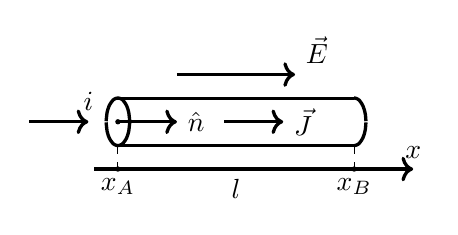
\begin{tikzpicture}[scale=1.5]
    \draw[->,very thick](-0.75,0)--(-0.25,0)node[above]{$i$};
    \draw[->,very thick](0,0)--(0.5,0)node[right]{$\hat{n}$};
    \filldraw[black](0,0)circle(0.5pt);
    \draw[->,very thick](0.9,0)--(1.4,0)node[right]{$\vec{J}$};
    \draw[->,very thick](0.5,0.4)--(1.5,0.4)node[above right]{$\vec{E}$};

    \draw[-,very thick]plot[smooth, domain=-0.1:0.1](\x,{(0.04-4*(\x)^2)^0.5});
    \draw[-,very thick]plot[smooth, domain=-0.1:0.1](\x,{-(0.04-4*(\x)^2)^0.5});
    \draw[-,very thick](0,0.2)--(2,0.2);
    \draw[-,very thick](0,-0.2)--(2,-0.2);
    \draw[-,very thick]plot[smooth, domain=2:2.1](\x,{(0.04-4*(\x-2)^2)^0.5});
    \draw[-,very thick]plot[smooth, domain=2:2.1](\x,{-(0.04-4*(\x-2)^2)^0.5});

    \draw[->,very thick](-0.2,-0.4)--(2.5,-0.4)node[above]{$x$};
    \draw[dashed](0,-0.2)--(0,-0.4)node[below]{$x_A$};
    \filldraw[black](0,-0.4)circle(0.5pt);
    \draw[dashed](2,-0.2)--(2,-0.4)node[below]{$x_B$};
    \filldraw[black](2,-0.4)circle(0.5pt);
    \node[below]at(1,-0.4){$l$};
\end{tikzpicture}
\end{document}